\documentclass[12pt,letterpaper]{article}

\usepackage{amsmath, amsthm, amsfonts, amssymb}
\usepackage{microtype, parskip, graphicx}
\usepackage[comma,numbers,sort&compress]{natbib}
\usepackage{lineno}
\usepackage{longtable}
\usepackage{docmute}
\usepackage{caption, subcaption, multirow, morefloats, rotating}
\usepackage{wrapfig}
\usepackage{hyperref}

\frenchspacing

\begin{document}

\section{Data Specifications}

We analyzed microfossil occurrence information which was downloaded from the Neptune Database \url{http://www.nsb-mfn-berlin.de/nannotax}. All occurrence information was downloaded for calcareous nannofossils, diatoms, foraminifera, and radiolarians -- these occurrences span the entire globe between 120 and 0 million years ago (Mya). This dataset of occurrences was then filtered to just those species which have their first occurrence at most 63 Mya. This choice means that our analysis avoids those taxa which survived the K/Pg boundary, those taxa which arose just after the K/Pg boundary, and means that our occurrence histories line up with the temperature time-series which was used as a predictor of extinction (discussed below).

All fossil occurrences were assigned to 1 My bins based on the estimated age of the fossil occurrence. Because the estimated ages of each occurrence is a product of core-specific age-models and can be overly precise, the hope is that by binning the data this smooths over the between-core heterogeneity and thus homogenizes our disparate data sources. The occurrence histories of each species were then given binary codes used to model the presence or extinction of those species. For every occurrence of a species, except the last, that species is considered to have survived and was marked with a 0. The last occurrence of that species is considered the bin in which the taxon has gone extinct -- and is assigned a 1. This protocol means that we are reading the fossil record ``as written,'' a practice that is potentially dangerous as it is a overconfident statement of preservation and may be shortening the actual duration of that species CITATIONS. However, this practice is common with marine microfossil data CITATIONS. In fact, with marine microfossils collected from cores a bigger problem may be over extending the duration of a species due to mixing and smearing within the cores CITATIONS.

A taxon's geographic range was calculated for each of the 1 My bins in which it occurred. Geographic range was calculated as the maximum great circle distance on an ellipsoid (i.e. the globe) between any two occurrences; this measure is also called a geodesic. This distance was measured in kilometers. The geodesic distance was then log-plus-one transformed and then standardized by zero-centering the data and then dividing by its standard deviation so that geographic range had mean 0 and standard deviation 1. This standardization means that a regression coefficient associated with this covariate describes the change in extinction probability per change in standard deviation of geographic range, and that coefficients associated with similarly standardized covariates will be directly comparable in magnitude \citep{ARM}.

Temperature data used as covariates in this analysis are based on Magnesium/Calcium isotope ratios sourced from \citet{Cramer2011}. These elemental ratios are considered more accurate estimates of past global temperature when compared to the frequently used Oxygen isotope-based estimates; this is because Mg/Ca based estimates are not effected by ice-volume and fresh-water input (e.g. meteoric water) which can alter Oxygen isotope ratios without reflecting changes to the climate itself. This property is of particular importance for this analysis as polar ice-caps develop midway through the Cenozoic. Our data source, \citet{Cramer2011}, provides temperature estimates for every 0.1 My from 0 to 63 Mya. We binned these estimates into 1 My intervals as we did with the fossil occurrences. The temperature estimate for each 1 My interval was calculated as the mean of all estimates within that interval (Fig. \ref{fig:temp_curve}). Temperature was then transformed and standardized the in the same manner as geographic range (above).

\begin{figure}[ht]
  \centering
  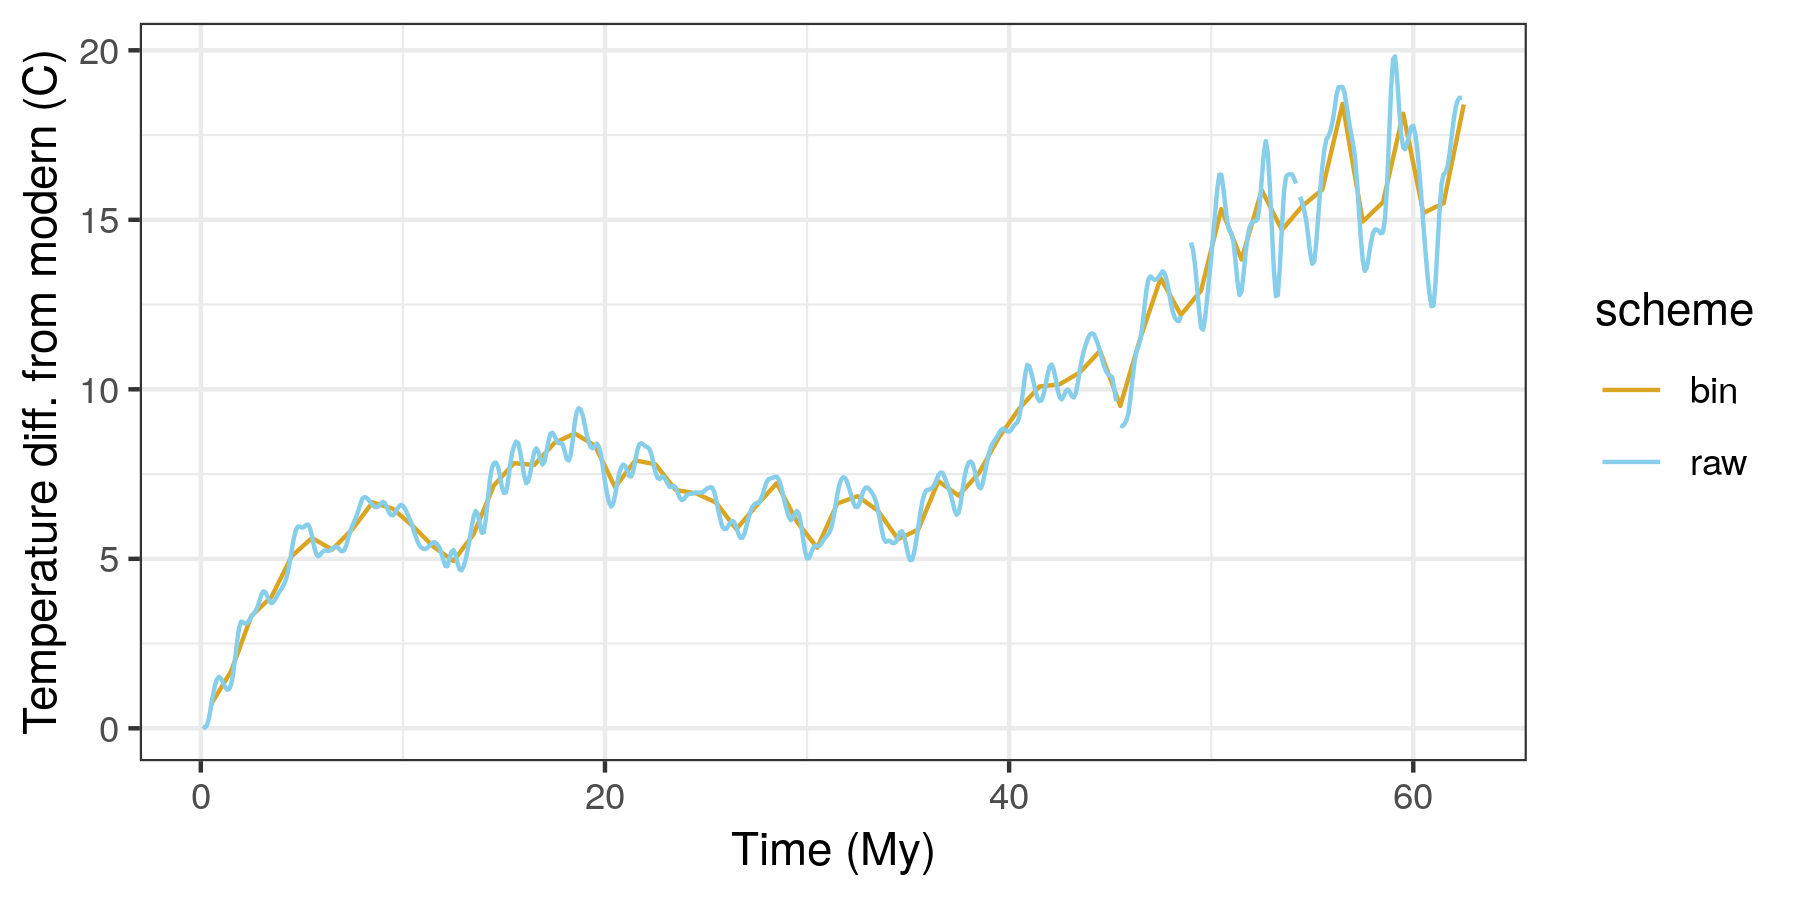
\includegraphics[width=\textwidth,height=0.5\textheight,keepaspectratio=true]{../results/figure/cramer_temp}
  \caption{Comparison of initial temperature estimates from Cramer et al. CITATION (goldenrod) versus the binned values used in this analysis (blue). The initial values are for every 0.1 My while our bins are defined for every 1 My.}
  \label{fig:temp_curve}
\end{figure}


\section{Model Specifications}

In survival analysis, the hazard function describes the instantaneous rate of extinction of a species given its age and relevant covariates. The hazard function is defined as the conditional probability of a species going extinct by the end of the \(t\)-th interval given that it survived up until \(t\) and the relevant covariate information \(X\) for all \(k\) 1 My intervals. For the discrete time intervals \(T = 1, \cdots, k\), extinction is defined as \(T = t\). The discrete time hazard function is defined as
\begin{equation}
  \lambda(t | X) = P(T = t | T \geq t, X), \quad t = 1, \cdots, k. \\
  \label{eq:hazard}
\end{equation}

The hazard function (Eq. \ref{eq:hazard}) is easily reparameterized as a logistic regression by defining that \(\lambda(t | X) = h(\Theta)\) where \(h(.)\) is a logit inverse-link function and \(\Theta\) is the probability of a taxon going extinction during interval \(t\). \(h(\Theta)\) is then modeled as with any regression as it is defined for all real-values. In this case, we opted for a hierarchical/mixed-effects model with multiple non-nested varying intercepts and slopes \citep{ARM}.

Our covariates matrix \(X\) is a \(N \times D\) matrix where \(N\) is the total number of observations and \(D\) is the total number of covariates. The first column of \(X\) is entirely 1's as it corresponds to the intercept term in the regression model. The next two columns of \(X\) are two aspects of geographic range as continuous covariates: geographic range \(r\) during interval \(t\), and the difference \(d\) between the geographic range at \(t - 1\) and \(t\). The difference in geographic range was calculated from the transformed and standardized geographic range values; this means that change in geographic range is in units of changes in standard deviations. The final two columns are two aspects of global temperature: mean temperature during interval \(t\), and the lag of mean temperature (i.e. mean temperature during interval \(t - 1\).) As with change to geographic range, the lag of temperature is based on the transformed and standardized temperature estimates. 

The matrix of time and phylum varying regression coefficients describing the effects of the covariates on a species' risk of extinction is called \(B\). These regression coefficients are themselves modeled as being multivariate normally distributed with vector of means \(\alpha\) describing the average intercept and regression coefficient estimates of each coefficients for each phylum \(p\). These phylum averages are themselves modeled as multivariate normally distributed with mean vector \(\mu\) describing the overall average regression coefficients, including the intercept. \(\mu\) has length \(D\) and is ordered intercept, range coefficient, change in range coefficient, temperature coefficient, temperature lag coefficient.

This logistic regression model, minus the final selection of priors, is expressed as 
\begin{equation}
  \begin{aligned}
    t_{i} &\sim \text{Bernoulli}(\Theta) \\
    \Theta_{i} &= \text{logit}^{-1} (X_{i} B_{w[i], p[i]} + A_{d[i], p[i]}) \\
    B_{w, p} &\sim MVN(\alpha_{p}, \Sigma_{B}) \\
    \alpha_{p} &\sim MVN(\mu, \Sigma_{\alpha}) \\
    % double check this\dots is A MVN dist?
    A_{w, p} &\sim MVN(\delta_{p}, \Sigma_{A}) \\
    \delta_{p} &\sim \mathrm{N}(0, \sigma_{\delta}) \\
  \end{aligned}
  \label{eq:core}
\end{equation}
with \(i\) indexing the observation and bracket subscripts referencing the class of the \(i\)th observation where \(w[i]\) is the time of the \(i\)-th observation, \(p[i]\) is the phylum of the \(i\)-th observation, and \(d[i]\) is the age of the \(i\)-th observation. 

To complete the generative model, we need to assign final priors to the ``top level'' parameters. In general we favored weakly informative priors which help regularize our estimates. In the case of a regression coefficient, this means a Normal distribution with mean 0 and a standard deviation of 3. For our scale parameters (e.g. standard deviations), we used half-Cauchy distributed priors with heavy tails but the majority of probability density near 0.

Our top-level intercept was given a more diffuse prior than our regression coefficients, which reflects our greater degree of uncertainty about its value. Our top-level regression coefficient for the effect of geographic range was given an informative prior reflecting the overwhelming amount of evidence that species with a larger than average geographic range have a lower risk of extinction than species with an average or less than average geographic range. In the context of this analysis, this means that we are again using a weakly informative prior but instead of centering the density around -1 (i.e. larger than average geographic range decreases extinction risk).

Instead of assigning a prior distribution for each of the covariance matrices in the model, we instead decomposed the covariance matrices (e.g. \(\Sigma_{B}\)) which allows us to assign independent priors for the scale and correlation aspects of covariance. The scale parameters were assigned half-Cauchy priors as described above in the context of all other scale parameters. The correlation matrices were assigned LKJ priors each with shape parameter set to 1. This choice of shape parameter produces a uniform distribution over possible correlation matrices. These priors are also slightly more interpretable than other common prior distributions for covariance matrices such as the inverse-Wishart distribution. This approach to assigning priors to a covariance matrix is recommended by the Stan Manual \citep{StanManual}.

In total, these prior choices can be expressed as
\begin{equation}
  \begin{aligned}
    \mu_{d} &\sim 
      \begin{cases}
        N(-2, 5) & \text{if } d = \text{intercept} \\
        N(-1, 1) & \text{if } d = \text{geo. range} \\
        N(0, 1) & \text{else } \\
      \end{cases}
    \delta &\sim N(0, 1) \\
    \Sigma_{B} &= diag(\tau_{B}) \Omega_{B} diag(\tau_{B}) \\
    \Sigma_{\alpha} &= diag(\tau_{\alpha}) \Omega_{\alpha} diag(\tau_{\alpha}) \\
    \Sigma_{A} &= diag(\tau_{A}) \Omega_{A} diag(\tau_{A}) \\
    \tau_{B} &\sim C^{+}(5) \\
    \tau_{\alpha} &\sim C^{+}(5) \\
    \tau_{A} &\sim C^{+}(5) \\
    \Omega_{B} &\sim LKJ(1) \\
    \Omega_{\alpha} &\sim LKJ(1) \\
    \Omega_{A} &\sim LKJ(1) \\
  \end{aligned}
  \label{eq:priors}
\end{equation}


We considered four variants of the model described above: 1) historical covariates with time-varying intercepts and slopes, 2) no historical coviarates with time-varying intercepts and slopes, 3) historical covariates without time-varying intercepts and slopes, and 4) no historical covariates and no time-varying intercepts and slopes (except age effect). The second and fourth models modify the number of columns in \(X\) by removing two of the covariates. The third and fourth model simplify the first model to just varying intercepts without varying slopes.


\section{Model Parameter Estimation}

We implemented our model using the \begin{texttt}rstanarm\end{texttt} package for the R programming language \citep{StanManual}. This package provides an interface to the Stan probabilistic programming language for writing hierarchical/mixed-effects models in native R. Posterior estimates were obtained through Hamiltonian Monte Carlo, using 2000 steps divided equally between warm-up and sampling. In order to prevent divergent transitions the adapt delta value was increased to 0.9999; all other HMC/NUTS sampling parameters were kept at the defaults for rstanarm 2.18.2 \citep{rstanarm}.

An implementation of our full model in \begin{texttt}rstanarm\end{texttt}, given a data.frame of all necessary data in a data.frame called ``data'', is coded as:
\begin{verbatim}
  stan_glmer(formula = event ~ range + range_diff + temp + temp_lag + 
                       (1 + range + range_diff + temp + temp_lag | mybin/phylum) + 
                       (1 | age/phylum), 
             data = data, 
             family = 'binomial',
             prior = normal(c(-1, 0, 0, 0), rep(1, 4), autoscale = FALSE), 
             prior_intercept = normal(0, 10, autoscale = FALSE), 
             prior_aux = cauchy(0, 3, autoscale = FALSE), 
             chains = 4,
             thin = 4,
             adapt_delta = 0.999999)
\end{verbatim}

Similarly, our full model can be implemented in \begin{texttt}brms\end{texttt} \citep{brms2017,brms2018} as:
\begin{verbatim}
priors <- c(set_prior('normal(0, 10)', class= 'Intercept'),
            set_prior('normal(0, 1)', class = 'b'),
            set_prior('normal(-1, 1)', class = 'b', coef = 'range'),
            set_prior('cauchy(0, 3)', class = 'sd'),
            set_prior('lkj(1)', class = 'cor'))
brmfit <- brm(formula = bf(event ~ range + range_diff + temp + temp_lag +
                           (1 + range + range_diff + temp + temp_lag | mybin/phylum) +
                           (1 | age/phylum))
              data = data, 
              family = bernoulli(), 
              prior = priors,
              chains = 4, 
              thin = 4,
              control = list(adapt_delta = 0.999999)
\end{verbatim}

Posterior convergence was determined using the general and HMC-specific diagnostic criteria: scale reduction factor (\(\hat{R}\); target \(<1.1\)), effective sample size (eff; target value eff/steps \(<0.0001\)), number of samples that saturated the maximum trajectory length for avoiding infinite loops (treedepth; target value 0), sample divergence, and the energy Bayesian Fraction of Mission Information (E-BFMI; target value \(>0.2\)). For further explanation of these diagnostic criteria, see the Stan Manual \citep{StanManual}.


\section{Model adequacy}

We are interested in model adequacy and performance into two contexts: in-sample and out-of-sample predictive performance. ``In-sample'' means we are estimating how well our model predicts our observed data given that the model was fit to the entire dataset; this is a posterior predictive check in that we are comparing the posterior predictive distribution to our observed data. ``Out-of-sample'' is defined below.

Relative and absolute model adequacy of the four variant models was compared using the area under the receiver operating characteristic curve (AUC). This measure is commonly used in classification problems as it has the desirable characteristic of comparing the model's true positive rate with its false positive rate, as opposed to accuracy which only considers the count of true positives. AUC ranges between 0.5 and 1, with 0.5 indicating no improvement in performance from random and 1 indicating perfect performance. 

The differences in in-sample predictive performance between the models was visualized in multiple ways: whole data set by model, taxonomic group by model, model performance over time, and model performance by taxonomic groups over time. These comparisons demonstrate the relative and absolute adequacy of the models in describing the dataset they were fit to.

We are particularly interested in understanding how well our model predicts species extinction given new, future data (out-of-sample data). To do this, we estimated average out-of-sample predictive error using 5-fold time-series cross-validation. For time-series data, the folds (data partitions) are approximately equal segments of time. The model is fit to the first fold and the posterior estimates are used to predict the states of the observations in the second fold, then the model is fit to the first and second fold and the posterior states are used to estimate the states from the third fold, and so on with increasingly large numbers of folds used for fitting a model to predict the states from the subsequent fold. With 63 time points, each of the five folds represents approximately 13 time points. Keep in mind, however, that each time point corresponds to many (100-1000) individual observations.


See our code repository LINK for full code details. Our code uses ``tidyverse'' tools such as dplyr \citep{dplyr}, purr \citep{purrr}, and tidybayes \citep{tidybayes}, thus some familiarity with that package ecosystem is necessary to fully comprehend how we've processed our data and results.


\end{document}
